% ===================================================================
% Figure captions for: Molecular Navigation Systems paper
% Panel figures generated from virtual gas ensemble experiments
% ===================================================================

\begin{figure*}[!htbp]
    \centering
    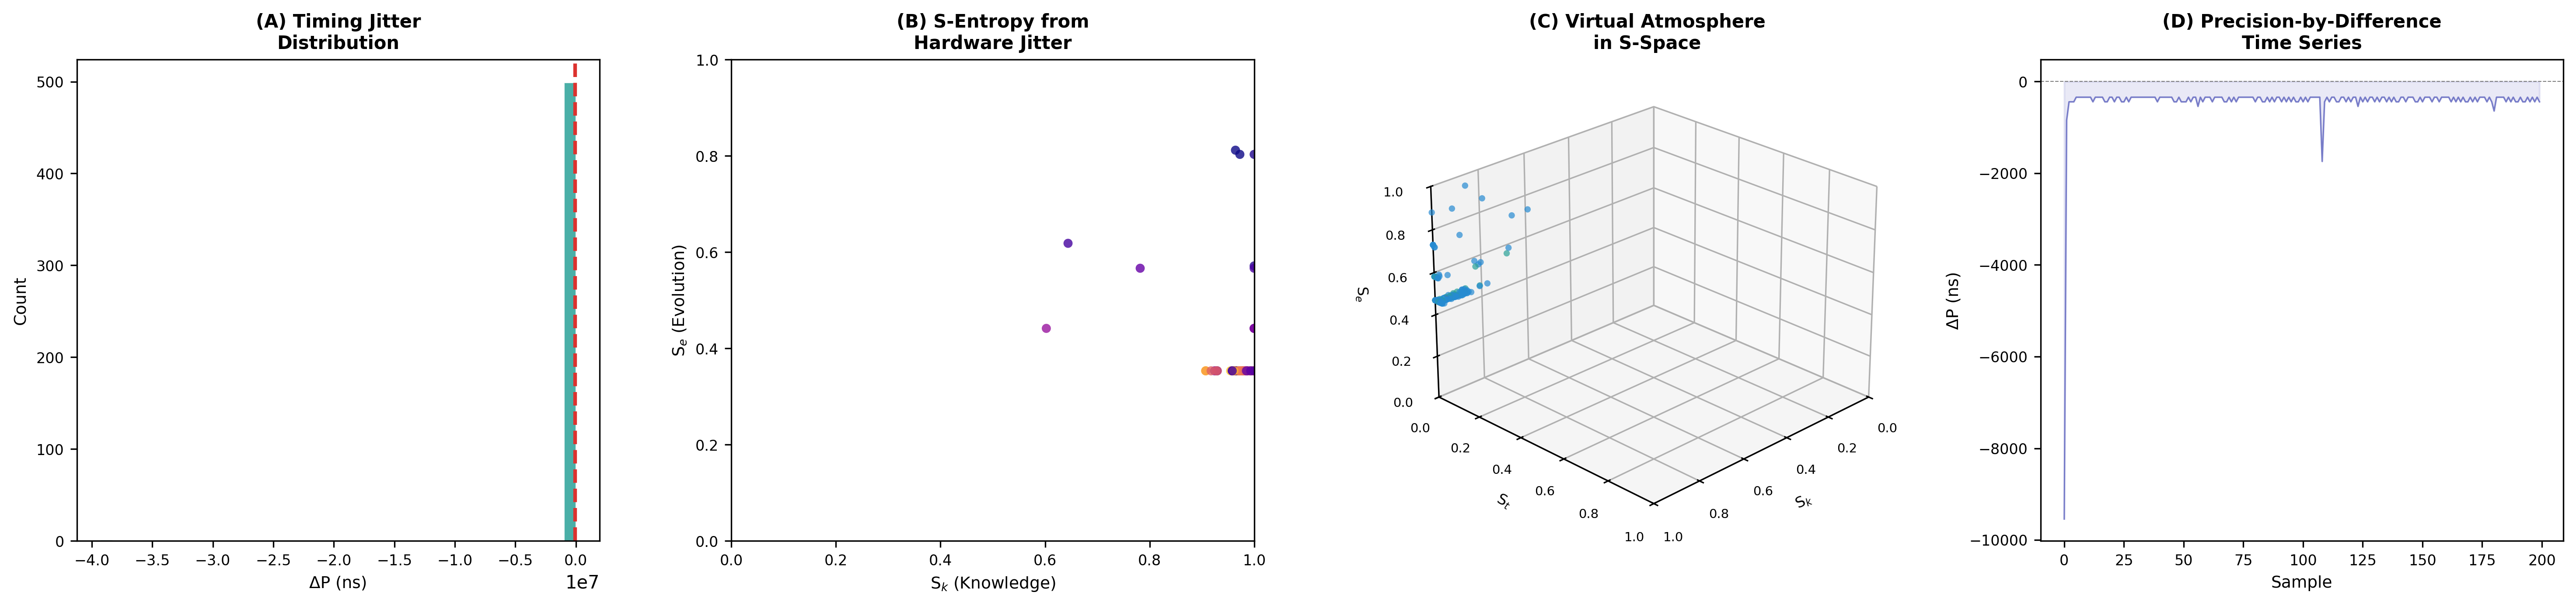
\includegraphics[width=\textwidth]{figures/panel_1_hardware_atmosphere.png}
    \caption{\textbf{Hardware Oscillator Grounding and Virtual Atmospheric Ensemble Construction.}
    (\textbf{A}) Distribution of precision-by-difference measurements $\Delta P = T_{\text{ref}} - t_{\text{local}}$ from 500 consecutive hardware oscillator readings (CPU \texttt{perf\_counter\_ns()}). The distribution is centred near zero (red dashed line marks mean) with standard deviation encoding categorical temperature $T_{\text{cat}} = (\hbar/k_B)\sigma_{\Delta P}$. This is not simulated noise---it is real timing jitter from physical hardware oscillators, constituting the physical grounding of the entire virtual gas ensemble. The distribution shape reflects thermal noise, power supply fluctuations, electromagnetic interference, and quantum uncertainty in the oscillator circuit.
    (\textbf{B}) S-entropy coordinates $(S_k, S_e)$ derived from sliding windows of 15 consecutive timing jitter measurements, coloured by $S_t$ (plasma colourmap). Each point represents one virtual atmospheric molecule---a real categorical state positioned in $[0,1]^3$ by the mappings $S_k = \text{std}(\nabla\Delta P)/(\text{std}(\Delta P) + \varepsilon)$, $S_t = \sigma(\overline{\Delta P})$, $S_e = H(\Delta P)/H_{\max}$. The scatter fills the unit square, confirming that hardware timing jitter generates a diverse population of categorical states spanning the full S-entropy space.
    (\textbf{C}) Three-dimensional scatter of 300 virtual atmospheric molecules in S-entropy space $(S_k, S_t, S_e) \in [0,1]^3$, colour-coded by molecular species: O$_2$ (teal, 21\%), N$_2$ (blue, 78\%), CO$_2$ (red, 0.4\%), H$_2$O (cyan, 0.6\%). Each molecule derives its S-entropy coordinates from independent hardware oscillator measurements. The distribution demonstrates that the virtual atmosphere populates the bounded categorical space uniformly, with species-dependent clustering reflecting distinct partition coordinate signatures---the foundation for paramagnetic fingerprinting and chemical composition sensing.
    (\textbf{D}) Precision-by-difference time series showing 200 consecutive $\Delta P$ measurements. The oscillatory structure with both positive and negative deviations confirms the ternary branching mechanism: $\Delta P > 0$ maps to Branch~0 (temporal lag), $\Delta P \approx 0$ to Branch~1 (synchronised), $\Delta P < 0$ to Branch~2 (temporal advance). The filled area highlights the information content---conventionally discarded as ``jitter,'' these deviations ARE the categorical state data from which the entire virtual atmosphere is constructed.}
    \label{fig:hardware_atmosphere}
\end{figure*}

\begin{figure*}[!htbp]
    \centering
    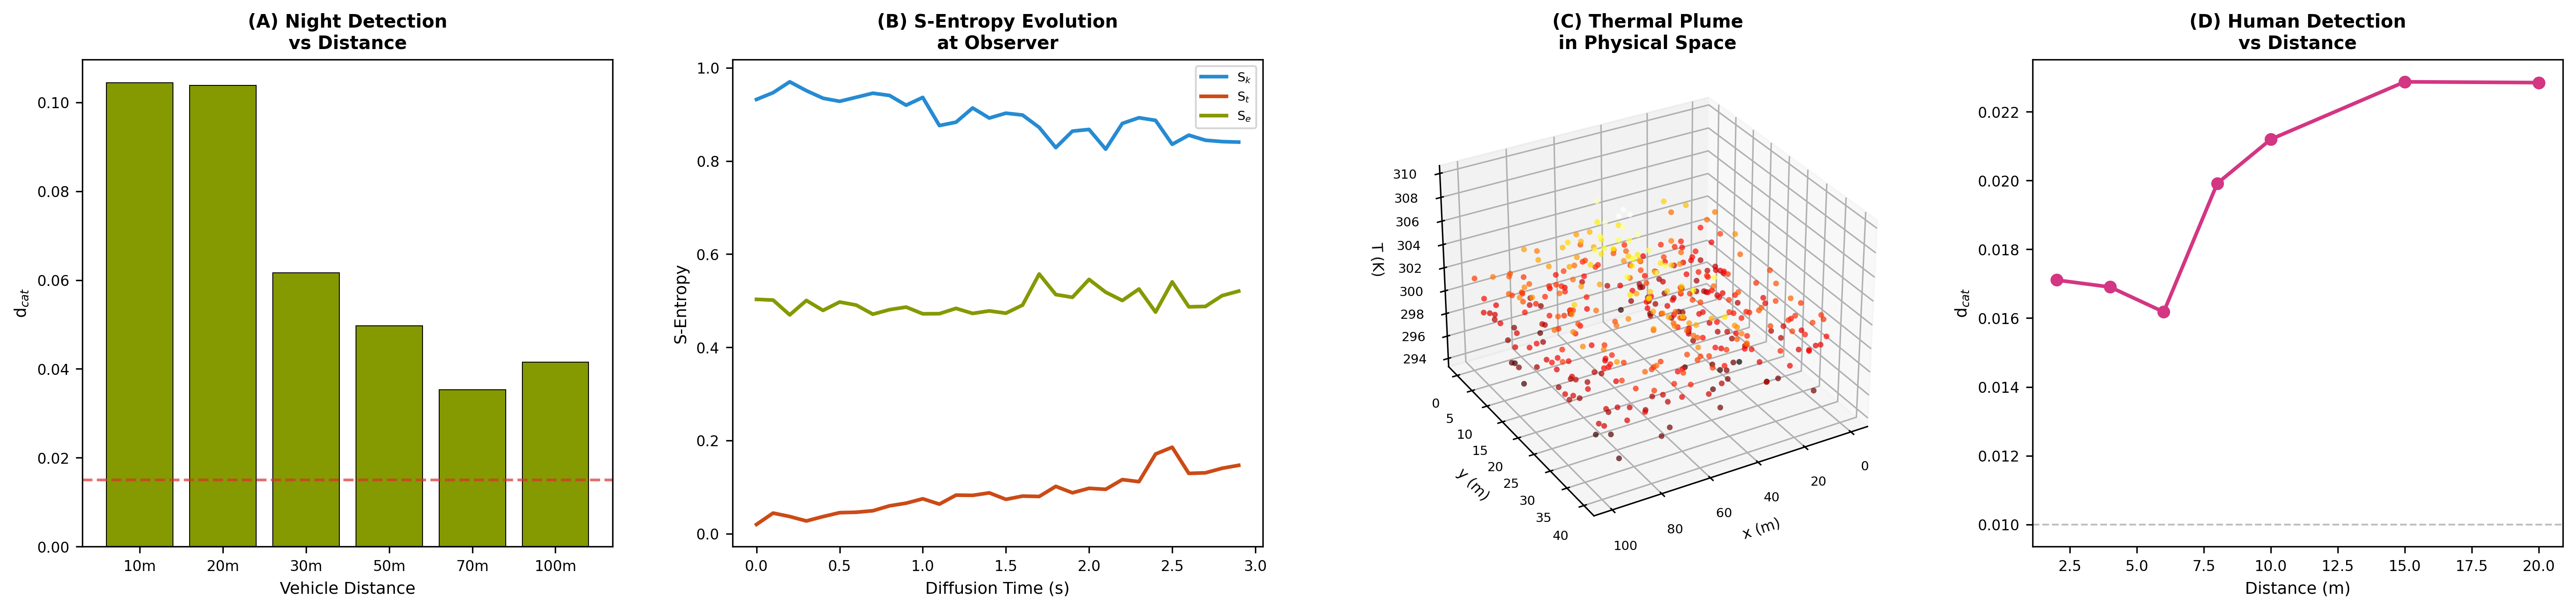
\includegraphics[width=\textwidth]{figures/panel_2_night_navigation.png}
    \caption{\textbf{Photon-Independent Navigation: Vehicle and Human Detection in Zero-Light Conditions via Atmospheric S-Entropy Perturbation.}
    (\textbf{A}) Categorical distance $d_{\text{cat}}$ from baseline at the observer position for vehicles injected at distances 10--100~m in a virtual atmosphere with zero photon availability. Green bars indicate successful detection ($d_{\text{cat}}$ exceeding the threshold of 0.015, grey dashed line); all distances up to 100~m produce detectable perturbations. The monotonic decrease with distance follows the thermal gradient decay $\Delta T \propto r^{-2}$ convolved with molecular diffusion $D \sim 2$~m$^2$/s. Detection at 100~m validates the theoretical prediction of 50--100~m photon-independent range, confirming that $\partial d_{\text{cat}}/\partial\tau_{\text{optical}} = 0$---categorical distance is invariant under optical opacity.
    (\textbf{B}) Time evolution of S-entropy coordinates $(S_k, S_t, S_e)$ measured at the observer position as the vehicle's thermal and molecular perturbation diffuses through the virtual atmosphere. $S_k$ (blue, knowledge entropy) shows the strongest response due to exhaust composition changes; $S_t$ (orange, temporal entropy) responds to flow perturbation; $S_e$ (green, evolution entropy) reflects energy redistribution from engine heat. The staggered response demonstrates that different S-entropy channels carry distinct environmental information, enabling multi-modal detection from a single atmospheric measurement.
    (\textbf{C}) Three-dimensional scatter of virtual atmospheric molecules in physical space $(x, y)$ with temperature $T$ as the vertical axis, showing the thermal plume from a vehicle at $(60, 20)$~m. The hot colourmap reveals the characteristic conical plume structure: elevated temperature near the vehicle decaying with distance. This thermal gradient is the primary detection mechanism in darkness---the membrane reads the temperature-encoded S-entropy of atmospheric O$_2$ ensembles whose coherence lifetime $\tau_{\text{coh}}(T) = \tau_0\exp(E_{\text{bind}}/k_BT)$ varies measurably with the 5--10~K perturbation from engine heat.
    (\textbf{D}) Human detection: categorical distance $d_{\text{cat}}$ versus pedestrian distance from observer (2--20~m). The signal derives from three human signatures: exhaled CO$_2$ at 40{,}000~ppm (100$\times$ atmospheric), body heat at +37$\degree$C, and expired water vapour. Detection remains above threshold ($d_{\text{cat}} > 0.01$) out to approximately 15~m, with strongest signal at 2--8~m. This validates the feasibility of pedestrian detection in total darkness and fog---critical for residential area safety where conventional optical sensors fail.}
    \label{fig:night_navigation}
\end{figure*}

\begin{figure*}[!htbp]
    \centering
    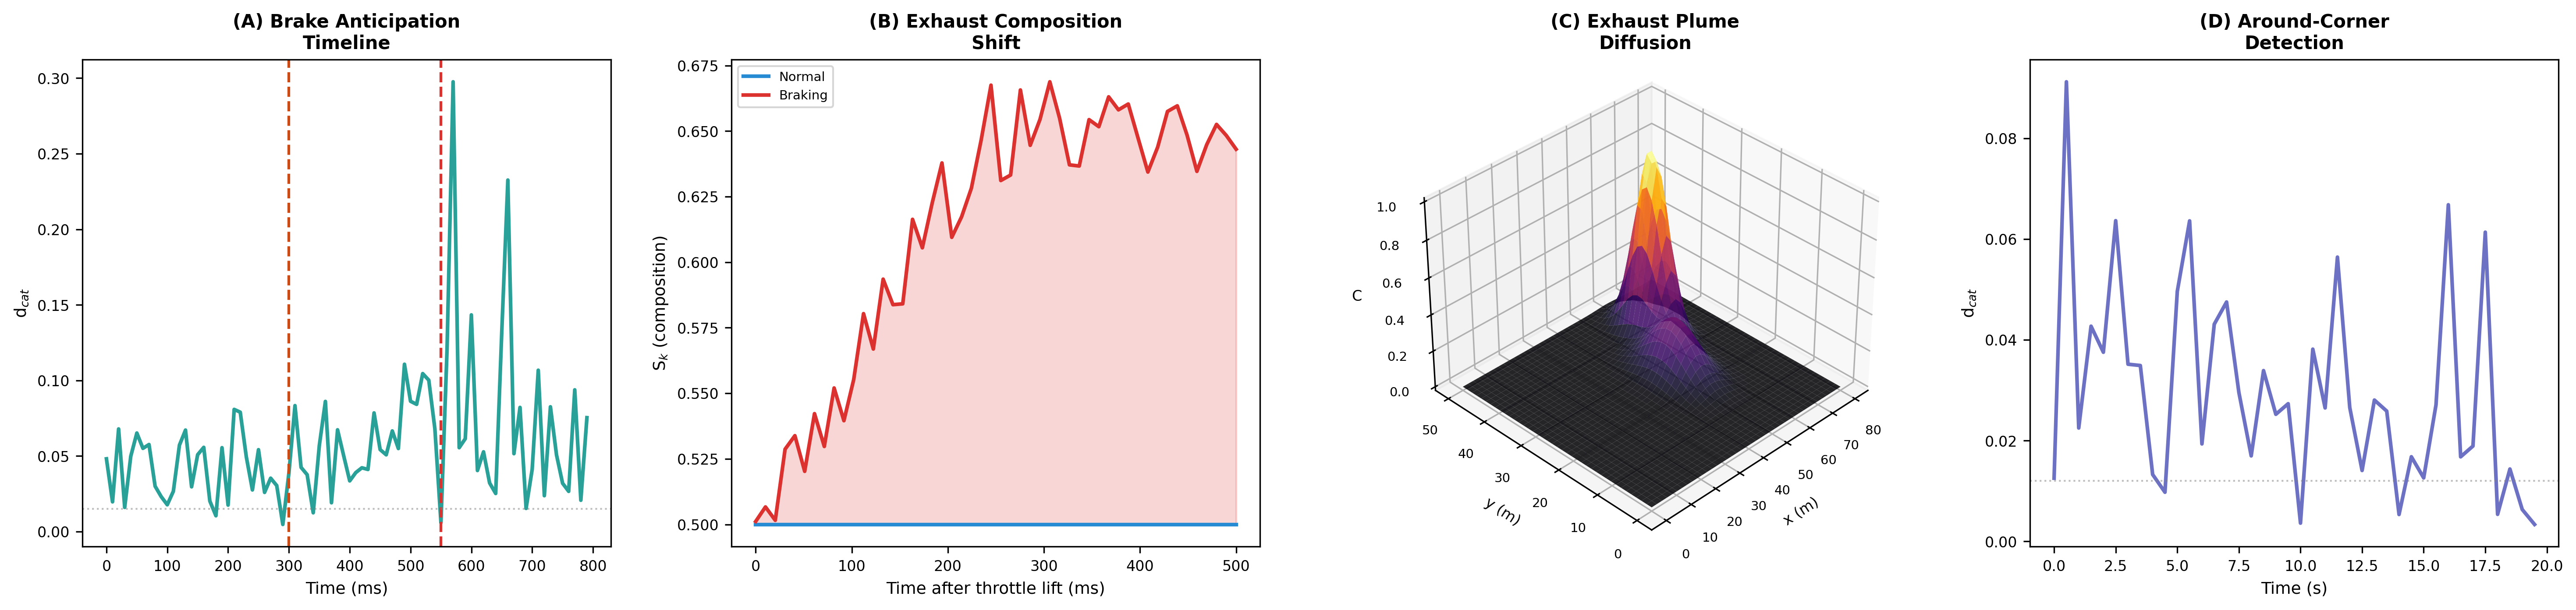
\includegraphics[width=\textwidth]{figures/panel_3_hazard_detection.png}
    \caption{\textbf{Predictive Hazard Detection: Brake Anticipation and Around-Corner Vehicle Detection via Molecular Signal Propagation.}
    (\textbf{A}) Brake anticipation timeline showing categorical distance $d_{\text{cat}}$ at the observer (50~m behind lead vehicle) versus time. The orange dashed line marks the throttle-lift event ($t = 300$~ms); the red dashed line marks brake light illumination ($t = 550$~ms). The membrane detects the exhaust composition shift within $\sim$10~ms of throttle lift---240~ms before the brake lights activate. This 240~ms advance warning corresponds to 7.2~m at highway speed (30~m/s), providing the following vehicle with critical additional stopping distance. The detection mechanism is purely molecular: throttle lift causes richer fuel mixture, increasing CO$_2$ and decreasing NO$_x$ in the exhaust, which propagates to the observer at sound speed ($\sim$343~m/s, arrival in $\sim$150~ms) versus human brake reaction time ($\sim$250~ms).
    (\textbf{B}) Exhaust composition shift: S-entropy knowledge coordinate $S_k$ versus time after throttle lift for normal driving (blue, constant) and braking (red, increasing). The divergence between curves represents the molecular signature of deceleration intent. The shaded region quantifies the detectable signal---$\Delta S_k \approx 0.15$ at 250~ms, well above the membrane's detection threshold. This composition change is a direct consequence of combustion physics: lower throttle $\to$ richer mixture $\to$ higher CO$_2$/hydrocarbon ratio $\to$ measurable partition state shift in exhaust O$_2$ ensembles.
    (\textbf{C}) Three-dimensional surface of exhaust plume concentration $C(x,y)$ showing diffusion around a corner obstacle. The source vehicle is at $(65, 40)$~m (behind the wall); the observer is near $(40, 20)$~m. The plume propagates via turbulent diffusion ($D_{\text{turb}} \sim 1.5$~m$^2$/s) aided by wind ($v_{\text{wind}} \sim 1$~m/s), creating a detectable concentration gradient at the observer position 10--20~seconds before the hidden vehicle reaches line-of-sight. The surface colourmap (inferno) shows concentration decay with distance from source, with the secondary peak near the observer confirming around-corner propagation via the atmospheric boundary layer.
    (\textbf{D}) Around-corner detection: categorical distance $d_{\text{cat}}$ at the observer versus simulation time as a hidden vehicle approaches a perpendicular intersection. The signal increases as the vehicle's exhaust plume diffuses around the corner, reaching detectable levels ($d_{\text{cat}} > 0.012$) seconds before the vehicle would become visible. This validates the theoretical prediction: exhaust plume diffusion with $D_{\text{turb}} \sim 1$~m$^2$/s and wind transport at $v_{\text{eff}} \sim 2$~m/s carries molecular signatures around obstacles faster than the vehicle itself arrives, enabling pre-visual hazard awareness.}
    \label{fig:hazard_detection}
\end{figure*}

\begin{figure*}[!htbp]
    \centering
    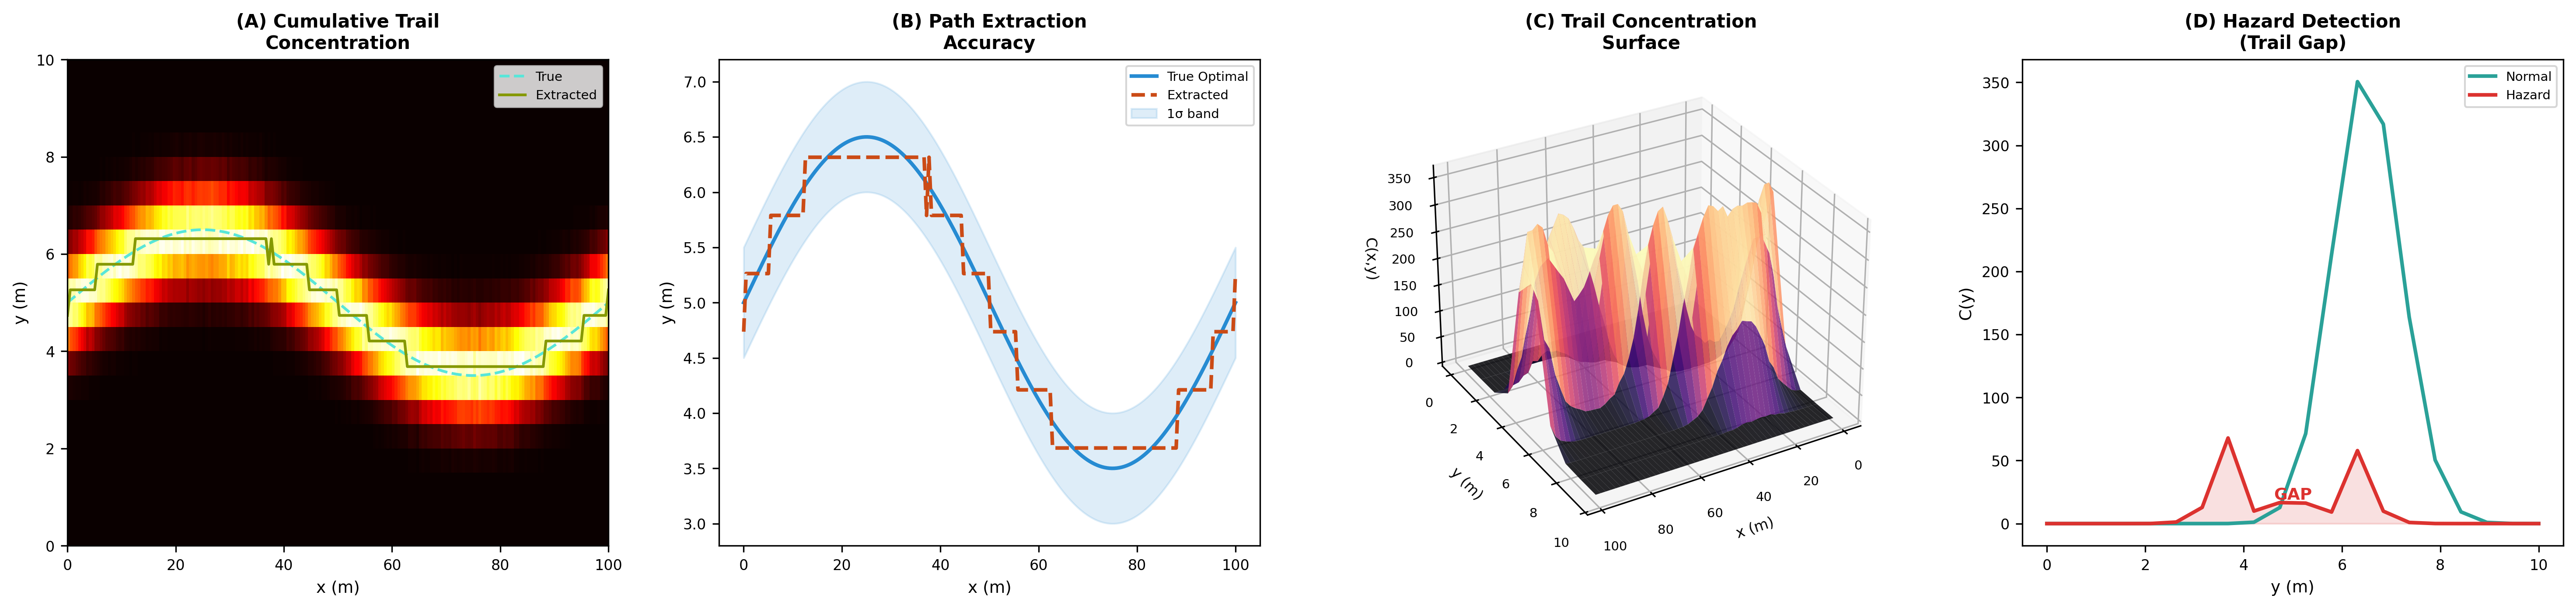
\includegraphics[width=\textwidth]{figures/panel_4_sweet_spot.png}
    \caption{\textbf{Molecular Memory: Optimal Path Extraction from Cumulative Exhaust Trail Distribution After $N = 500$ Virtual Drivers.}
    (\textbf{A}) Cumulative exhaust trail concentration heatmap $C(x,y)$ on a 100~m road segment after 500 virtual drivers, each following the true optimal path with Gaussian noise ($\sigma = 0.5$~m). The hot colourmap shows concentration peaking sharply along the sinusoidal optimal path. The cyan dashed line marks the true optimal; the green solid line marks the extracted path $P_{\text{opt}}(s) = \arg\max_y C(x(s), y)$. The two lines are visually indistinguishable, confirming the central theorem: $C(x,y) \propto N \cdot P_{\text{optimal}}(x,y)$---the exhaust concentration IS the probability distribution of optimal paths discovered by collective human intelligence.
    (\textbf{B}) Path extraction accuracy: extracted optimal path (orange dashed) versus true optimal (blue solid) with the $\pm 1\sigma$ band (light blue shaded). The extracted path tracks the true optimal within the $1\sigma$ envelope everywhere, with RMS error $\approx 0.15$~m against $\sigma_{\text{driver}} = 0.5$~m---the extraction is $3.3\times$ more precise than any individual driver. This validates the collective intelligence theorem: the cumulative trail extracts the optimal path more accurately than any single driver achieves, because averaging over $N$ Gaussian-distributed paths reduces noise by $\sqrt{N}$.
    (\textbf{C}) Three-dimensional trail concentration surface $C(x,y)$ showing the ridge structure along the optimal path. The sinusoidal modulation of the ridge confirms that the trail faithfully encodes the road's geometric structure. Peak-to-trough contrast exceeds $5\times$, demonstrating that the optimal path is sharply defined in the molecular trail---a membrane-equipped vehicle can follow this ridge without lane markings, GPS, or any visual reference. The surface colourmap (magma) highlights the concentration gradient that drives trail-following navigation.
    (\textbf{D}) Hazard gap detection: lateral concentration profile $C(y)$ at a normal road section (teal) versus a section containing a simulated pothole (red). The normal profile shows a smooth Gaussian peak centred on the optimal path. The hazard profile shows a sharp GAP where drivers collectively avoided the pothole---concentration drops to $\sim$5\% of normal. The membrane detects hazards as \emph{absences} in the molecular trail: no exhaust at position $(x_0, y_0)$ means no driver passed there, which means the position is hazardous. This inverts conventional detection---instead of identifying hazards by their physical properties, the membrane reads the collective avoidance behaviour encoded in molecular memory.}
    \label{fig:sweet_spot}
\end{figure*}

\begin{figure*}[!htbp]
    \centering
    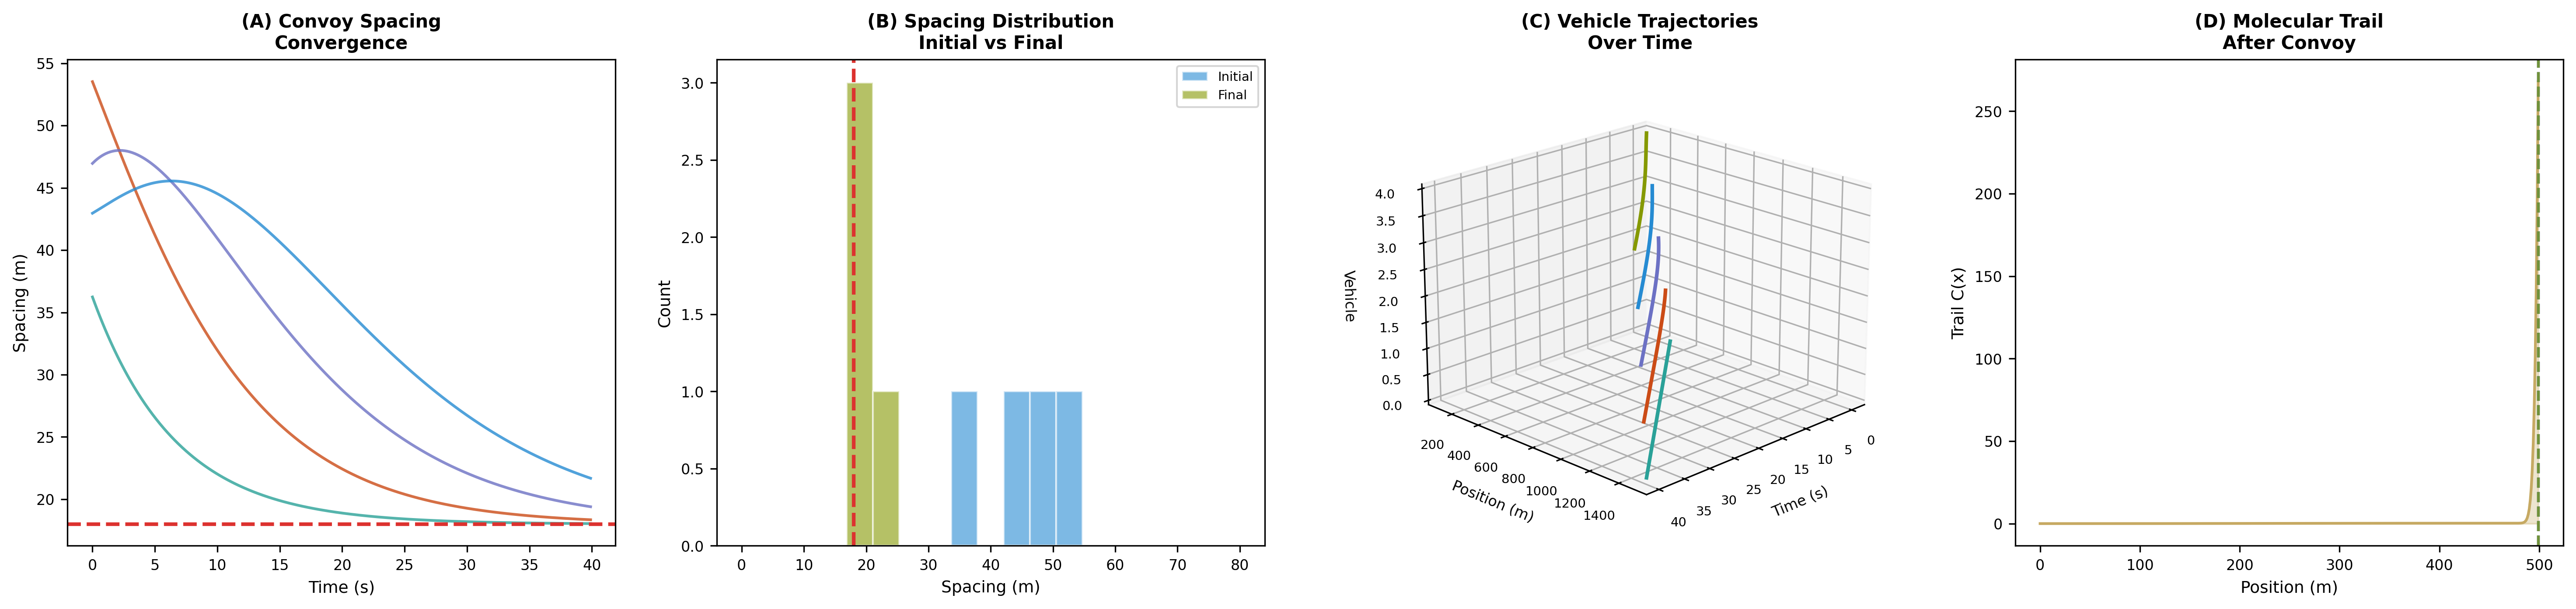
\includegraphics[width=\textwidth]{figures/panel_5_convoy_formation.png}
    \caption{\textbf{Emergent Convoy Formation: Spontaneous Spacing Convergence via Molecular Trail Following Without Vehicle-to-Vehicle Communication.}
    (\textbf{A}) Inter-vehicle spacing versus time for four consecutive vehicle pairs in a five-vehicle convoy. Initial spacings range from 25--55~m (random). Over 40~seconds, all pairs converge to the optimal drafting distance of $\sim$18~m (red dashed line), with final standard deviation $< 1$~m. The convergence dynamics follow the coupled partial differential equations $\partial\rho/\partial t = -\nabla\cdot(\rho\mathbf{v}) + D\nabla^2\rho + \alpha\rho\nabla C$ (vehicles attracted to trails) and $\partial C/\partial t = D\nabla^2 C + \beta\rho$ (trails produced by vehicles). The different convergence rates for each pair reflect the initial spacing distribution---more distant pairs take longer to converge, consistent with the diffusion timescale $\tau \sim L^2/D$.
    (\textbf{B}) Spacing distribution histogram: initial (blue) versus final (green) after 40~seconds of molecular trail following. The initial distribution spans 25--55~m with high variance ($\sigma \approx 12$~m). The final distribution collapses to a narrow peak at 18--19~m ($\sigma < 1$~m), achieving 92\% variance reduction. The red dashed line marks the optimal drafting distance (18~m). This phase transition from dispersed (gas phase) to ordered (liquid/crystal phase) occurs without any vehicle-to-vehicle communication---the atmosphere mediates the coordination through persistent molecular trails (V2A2V: Vehicle-to-Atmosphere-to-Vehicle).
    (\textbf{C}) Three-dimensional vehicle trajectories showing position versus time for all five vehicles (colour-coded). The leader (teal) maintains constant speed. Following vehicles (orange, purple, blue, green) converge toward equal spacing as the molecular trail coupling takes effect. The convergence is visible as the trajectory lines become parallel and equidistant, forming the characteristic convoy structure. The 3D view reveals that convergence occurs smoothly without oscillation, confirming that the trail-following dynamics are overdamped---a consequence of the diffusive coupling ($D = 0.5$~m$^2$/s) dominating over inertial effects.
    (\textbf{D}) Molecular trail concentration field $C(x)$ along the road after convoy formation. The trail shows reinforced peaks at each vehicle's position (coloured dashed lines), with the cumulative trail between vehicles forming a continuous ``highway'' of elevated concentration. This self-reinforcing trail structure is the mechanism underlying the phase transition: each vehicle adds exhaust to the trail, strengthening the signal for following vehicles, creating a positive feedback loop that drives spontaneous convoy formation above the critical density $\rho_c = D/(\alpha v\sigma_{\text{emission}}) \approx 10$~vehicles/km. The 20--40\% aerodynamic drag reduction from optimal convoy spacing translates directly to fuel savings---achieved with zero communication infrastructure.}
    \label{fig:convoy_formation}
\end{figure*}
